\documentclass{beamer}

\usepackage{amsfonts,amsbsy,amsthm,amsmath,amssymb}
\usepackage{listings}

\DeclareMathOperator*{\argmax}{arg\,max}
\DeclareMathOperator*{\argmin}{arg\,min}
\DeclareMathOperator{\ord}{ord}
\DeclareMathOperator{\sign}{sign}

\newcommand{\CC}{\mathbb{C}}
\newcommand{\NN}{\mathbb{N}}
\newcommand{\RR}{\mathbb{R}}
\newcommand{\ZZ}{\mathbb{Z}}
\newcommand{\QQ}{\mathbb{Q}}
\newcommand{\RRgtz}{\mathbb{R}_{>0}}
\newcommand{\ZZgtz}{\mathbb{Z}_{>0}}
\newcommand{\ZZgez}{\mathbb{Z}_{\ge 0}}
\newcommand{\QQgtz}{\mathbb{Q}_{>0}}
\newcommand{\QQgez}{\mathbb{Q}_{\ge 0}}

\newcommand{\KK}{\mathcal{K}}
\newcommand{\MM}{\mathcal{M}}
\newcommand{\OO}{\mathcal{O}}

\newcommand{\matrixto}[2]{\left[ \begin{array}{rr} #1 & #2 \end{array} \right]}
\newcommand{\matrixot}[2]{\left[ \begin{array}{r} #1 \\ #2 \end{array} \right]}
\newcommand{\matrixtt}[4]{\left[ \begin{array}{rr} #1 & #2 \\ #3 & #4 \end{array} \right]}
\newcommand{\matrixltt}[4]{\left[ \begin{array}{ll} #1 & #2 \\ #3 & #4 \end{array} \right]}
\newcommand{\matrixThreeOne}[3]{\left[ \begin{array}{rrr} #1 & #2 & #3 \end{array} \right]}
\newcommand{\matrixThreeTwo}[6]{\left[ \begin{array}{rrr} #1 & #2 & #3 \\ #4 & #5 & #6 \end{array} \right]}
\newcommand{\ntoinfty}{\lim_{n \rightarrow \infty}}
\newcommand{\floor}[1]{\left\lfloor #1 \right\rfloor}
\newcommand{\ceil}[1]{\left\lceil #1 \right\rceil}

\newcommand{\band}{~\texttt{and}_\texttt{2}~}
\newcommand{\bor}{~\texttt{or}_\texttt{2}~}
\newcommand{\bxor}{\oplus}
\newcommand{\bnot}{\lnot}
\newcommand{\binary}[1]{\texttt{#1}_\texttt{2}}

\newcommand{\set}{\mathcal}
\newcommand{\ideal}{\mathfrak}
\newcommand{\idealclass}[1]{\left[ \ideal #1 \right]}
\newcommand{\aclass}{\idealclass a}
\newcommand{\bclass}{\idealclass b}
\newcommand{\cclass}{\idealclass c}
\newcommand{\dclass}{\idealclass d}
\newcommand{\pclass}{\idealclass p}
\newcommand{\qclass}{\idealclass q}
\newcommand{\idclass}{[\mathcal O_\Delta]}
\newcommand{\hdelta}{\sqrt{|\Delta|}}

\newcommand{\hash}{\textrm{hash}_{\textrm{32}}}

\newcommand{\ith}{i^{\textrm{th}}}

\newcommand{\mygraph}[3]{
	\begin{figure}[htb]
	\centering
	\includegraphics{#1}
	\caption{#3}
	\label{#2}
	\end{figure}
}

% Same as \mygraph only it allows for a custom TOC description.
\newcommand{\mygraphX}[4]{
	\begin{figure}[htb]
	\centering
	\includegraphics{#1}
	\caption[#4]{#3}
	\label{#2}
	\end{figure}
}

\newcommand{\mygraphXPNG}[4]{
	\begin{figure}[htb]
	\centering
	\includegraphics[scale=0.5]{#1}
	\caption[#4]{#3}
	\label{#2}
	\end{figure}
}

\newcommand{\mygraphTwo}[4]{
	\begin{figure}[htb]
	\centering
	\includegraphics{#1}
	\includegraphics{#2}
	\caption{#4}
	\label{#3}
	\end{figure}
}

% Same as \mygraphTwo, but allows for a custom TOC desc.
\newcommand{\mygraphTwoX}[5]{
	\begin{figure}[htb]
	\centering
	\includegraphics{#1}
	\includegraphics{#2}
	\caption[#5]{#4}
	\label{#3}
	\end{figure}
}

\graphicspath{{eps/}}

\title[Ideal Class Group]{Improved Arithmetic in the Ideal Class Group of Imaginary Quadratic Number Fields}
\subtitle{With an Application to Integer Factoring}
\author{Maxwell Sayles}
\date{May 22, 2013}
\institute{
	\bigskip 
       Department of Computer Science \\
       University of Calgary
}

\usetheme{Copenhagen}
\usecolortheme{orchid}
%\setbeamertemplate{footline}[frame number]
% TODO: slide numbers


% What's important is to state and motivate the topic, highlight/outline your original results and contributions, give an overview of your methodology, assess significance, and give some interesting future work.  

%Ideal Class Group - NUCOMP, NUDUPL, NUCUBE... XGCD
%Exponentiation - 2,3 number system. L2R and Tree based.
%SPAR

%Improvements:
%- XGCD
%- left-to-right best approximations
%- SuperSPAR


\begin{document}
\maketitle

% OVERVIEW
\begin{frame}
\frametitle{Overview}

Major goals:
\begin{itemize}
\item Improve the performance of arithmetic in the ideal class group of imaginary quadratic number fields.
\item An optimized implementation of the SuperSPAR integer factoring algorithm.
\end{itemize}

\end{frame}

% MAJOR CONTRIBUTIONS
\begin{frame}
\frametitle{Major Contributions}
\begin{itemize} %[<+->]
\item An implementation of arithmetic in the ideal class group of imaginary quadratic number fields.
\item A method for generating 2,3 representations useful for exponentiation by power primorials.
\item A new integer factoring algorithm with implementation.
\end{itemize}
\end{frame}
  
% IDEAL CLASS IMPL
\begin{frame}
\frametitle{Arithmetic in the Ideal Class Group}
\begin{itemize}
\item Specialized implementations for 64-bit and 128-bit discriminants.
\item Improves upon Pari for discriminants smaller than 140-bits.
\end{itemize}
\end{frame}  
  
% XGCD
\begin{frame}
\frametitle{Extended Greatest Common Divisor}
Compute solutions to equations of the form
\[
	s = Ua + Vb = \gcd(a, b).
\]

\begin{itemize}
\item Specialized implementations for 32-bit, 64-bit, and 128-bit words.
\end{itemize}

\end{frame}

% XGCD Experiments
\begin{frame}
\frametitle{Extended Greatest Common Divisor Experiments}
TODO: A lare set of random numbers
\end{frame}

% XGCD Results
\begin{frame}
\frametitle{Extended Greatest Common Divisor Results}
TODO: Insert picture
\end{frame}

% IDEAL CLASS GROUP EXPERIMENTS
\begin{frame}
\frametitle{Ideal Class Group Experiments}
TODO: Took about a day
\end{frame}

% IDEAL CLASS GROUP RESULTS
\begin{frame}
\frametitle{Ideal Class Group Results}
TODO: insert pretty picture
\end{frame}

% EXPONENTIATION
\begin{frame}
\frametitle{Exponentiation by Odd Power Primorials}
The goal is to compute
\[
\aclass ^ E
\]
for some ideal class $\aclass$ and exponent
\[
	E = \prod_{i=2}^k {p_i}^{e_i}
\]
where $p_i$ is the $\ith$ prime.
\end{frame}

% L2R BEST APPROXIMATIONS
\begin{frame}
\frametitle{Left-to-Right Best Approximations}
Compute the set of best $2^a3^b$ approximations and only keep the $L$ best leaves.
\end{frame}

% EXPONENTIATION EXPERIMENTS
\begin{frame}
\frametitle{Exponentiation Experiments}
TODO: Use results of ideal class group arithmetic experiments to estimate the cost of each
\begin{itemize}
\item Faster.  Each time we change XGCD, we re-time arithmetic, not necessary to retime exponentiation.
\end{itemize}
\end{frame}

% EXPONENTIATION RESULTS (64)
\begin{frame}
\frametitle{Exponentiation Results (64-bit Implementation)}

\begin{figure}
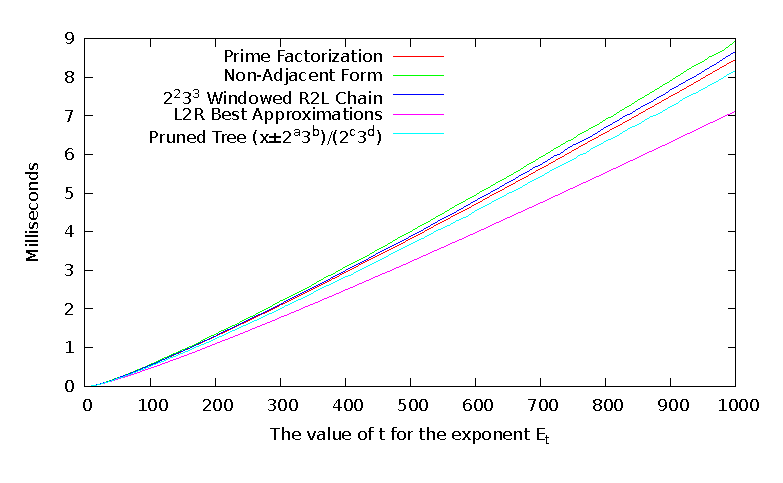
\includegraphics[scale=0.86]{winners-64}
\end{figure}

\end{frame}

% EXPONENTIATION RESULTS (128)
\begin{frame}
\frametitle{Exponentiation Results (128-bit Implementation)}

\begin{figure}
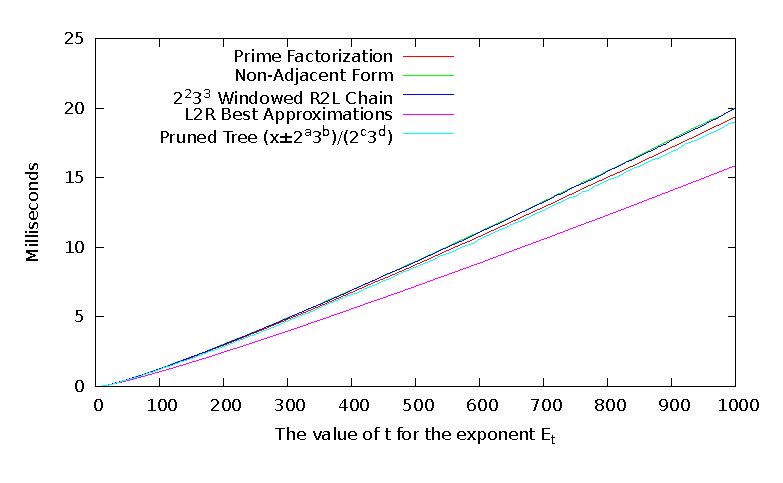
\includegraphics[scale=0.86]{winners-128}
\end{figure}

\end{frame}

% SUPERSPAR
\begin{frame}
\frametitle{SuperSPAR}

SuperSPAR is an integer factoring algorithm based on arithmetic in the ideal class group of imaginary quadratic integers.
\begin{itemize}
\item Extension of SPAR 
\end{itemize}

\end{frame}


\end{document}

